% **************************************************************************************************************
% A Classic Thesis Style
% An Homage to The Elements of Typographic Style
%
% Copyright (C) 2018 André Miede and Ivo Pletikosić
%
% If you like the style then I would appreciate a postcard. My address
% can be found in the file ClassicThesis.pdf. A collection of the
% postcards I received so far is available online at
% http://postcards.miede.de
%
% License:
% This program is free software; you can redistribute it and/or modify
% it under the terms of the GNU General Public License as published by
% the Free Software Foundation; either version 2 of the License, or
% (at your option) any later version.
%
% This program is distributed in the hope that it will be useful,
% but WITHOUT ANY WARRANTY; without even the implied warranty of
% MERCHANTABILITY or FITNESS FOR A PARTICULAR PURPOSE.  See the
% GNU General Public License for more details.
%
% You should have received a copy of the GNU General Public License
% along with this program; see the file COPYING.  If not, write to
% the Free Software Foundation, Inc., 59 Temple Place - Suite 330,
% Boston, MA 02111-1307, USA.
%
% PLEASE SEE ALSO THE AUTHORS' NOTE REGARDING THIS LICENSE
% IN THE DOCUMENTATION (ClassicThesis.pdf --> Chapter 1 / Chapter01.tex)
% **************************************************************************************************************
\RequirePackage{silence} % :-\
    \WarningFilter{scrreprt}{Usage of package `titlesec'}
    %\WarningFilter{scrreprt}{Activating an ugly workaround}
    \WarningFilter{titlesec}{Non standard sectioning command detected}
\documentclass[ oneside,openany,titlepage,numbers=noenddot, headinclude,
                % added by lexy
                % footinclude,1headlines,
                cleardoublepage=empty,abstract=on,
                BCOR=5mm,paper=a4,fontsize=10pt
                ]{scrreprt}

%********************************************************************
% Note: Make all your adjustments in here
%*******************************************************
% ****************************************************************************************************
% classicthesis-config.tex
% formerly known as loadpackages.sty, classicthesis-ldpkg.sty, and classicthesis-preamble.sty
% Use it at the beginning of your ClassicThesis.tex, or as a LaTeX Preamble
% in your ClassicThesis.{tex,lyx} with % ****************************************************************************************************
% classicthesis-config.tex
% formerly known as loadpackages.sty, classicthesis-ldpkg.sty, and classicthesis-preamble.sty
% Use it at the beginning of your ClassicThesis.tex, or as a LaTeX Preamble
% in your ClassicThesis.{tex,lyx} with % ****************************************************************************************************
% classicthesis-config.tex
% formerly known as loadpackages.sty, classicthesis-ldpkg.sty, and classicthesis-preamble.sty
% Use it at the beginning of your ClassicThesis.tex, or as a LaTeX Preamble
% in your ClassicThesis.{tex,lyx} with \input{classicthesis-config}
% ****************************************************************************************************
% If you like the classicthesis, then I would appreciate a postcard.
% My address can be found in the file ClassicThesis.pdf. A collection
% of the postcards I received so far is available online at
% http://postcards.miede.de
% ****************************************************************************************************


% ****************************************************************************************************
% 0. Set the encoding of your files. UTF-8 is the only sensible encoding nowadays. If you can't read
% äöüßáéçèê∂åëæƒÏ€ then change the encoding setting in your editor, not the line below. If your editor
% does not support utf8 use another editor!
% ****************************************************************************************************
\PassOptionsToPackage{utf8}{inputenc}
  \usepackage{inputenc}

\PassOptionsToPackage{T1}{fontenc} % T2A for cyrillics
  \usepackage{fontenc}


% ****************************************************************************************************
% 1. Configure classicthesis for your needs here, e.g., remove "drafting" below
% in order to deactivate the time-stamp on the pages
% (see ClassicThesis.pdf for more information):
% ****************************************************************************************************
\PassOptionsToPackage{
  drafting=false,    % print version information on the bottom of the pages
  tocaligned=false, % the left column of the toc will be aligned (no indentation)
  dottedtoc=true,  % page numbers in ToC flushed right
  eulerchapternumbers=false, % use AMS Euler for chapter font (otherwise Palatino)
  linedheaders=false,       % chaper headers will have line above and beneath
  floatperchapter=true,     % numbering per chapter for all floats (i.e., Figure 1.1)
  eulermath=false,  % use awesome Euler fonts for mathematical formulae (only with pdfLaTeX)
  beramono=true,    % toggle a nice monospaced font (w/ bold)
  palatino=true,    % deactivate standard font for loading another one, see the last section at the end of this file for suggestions
  style=classicthesis % classicthesis, arsclassica
}{classicthesis}


% ****************************************************************************************************
% 2. Personal data and user ad-hoc commands (insert your own data here)
% ****************************************************************************************************
\newcommand{\myTitle}{My Very Awesome And Ground Breaking Thesis}
\newcommand{\mySubtitle}{An Homage to The Elements of Typographic Style\xspace}
\newcommand{\myDegree}{Doctor of Philosophy\xspace}
\newcommand{\myName}{A. N. Other\xspace}
\newcommand{\myProf}{Prof Mojo Jojo\xspace}
\newcommand{\myOtherProf}{Dr Dexter Mandark\xspace}
% \newcommand{\mySupervisor}{Dr Sphesihle Makhathini\xspace}
\newcommand{\myFaculty}{\href{https://ratt.center}{Centre for Radio Astronomy Techniques and Technologies}\xspace}
\newcommand{\myDepartment}{\href{https://www.ru.ac.za/physicsandelectronics/}{Department of Physics and Electronics}\xspace}
\newcommand{\myUni}{Rhodes University\xspace}
\newcommand{\myLocation}{Makhanda\xspace}
\newcommand{\myTime}{\today\xspace}
\newcommand{\myVersion}{v1.0}

% ********************************************************************
% Setup, finetuning, and useful commands
% ********************************************************************
\providecommand{\mLyX}{L\kern-.1667em\lower.25em\hbox{Y}\kern-.125emX\@}
\newcommand{\ie}{i.\,e.}
\newcommand{\Ie}{I.\,e.}
\newcommand{\eg}{e.\,g.}
\newcommand{\Eg}{E.\,g.}
% ****************************************************************************************************


% ****************************************************************************************************
% 3. Loading some handy packages
% ****************************************************************************************************
% ********************************************************************
% Packages with options that might require adjustments
% ********************************************************************
\PassOptionsToPackage{british}{babel} % change this to your language(s), main language last
% Spanish languages need extra options in order to work with this template
%\PassOptionsToPackage{spanish,es-lcroman}{babel}
    \usepackage{babel}

\usepackage{csquotes}
\PassOptionsToPackage{%
  % backend=biber,bibencoding=utf8, uniquename=false, uniquelist=false,%instead of bibtex
  backend=bibtex8, bibencoding=ascii,%
  language=auto,%
  style=authoryear,%
  % style=authoryear-comp, % Author 1999, 2010
  %bibstyle=authoryear,dashed=false, % dashed: substitute rep. author with ---
  sorting=nyt, % name, year, title
  maxbibnames=3, % default: 3, et al.
  maxcitenames=2,
  %backref=true,%
  natbib=true, % natbib compatibility mode (\citep and \citet still work),
 % sortcites=true
}{biblatex}
    \usepackage{biblatex}
    \setlength\bibitemsep{\baselineskip}
% \AtBeginRefsection{\GenRefcontextData{sorting=nyt}}
% \AtEveryCite{\localrefcontext[sorting=ynt]}

% Lexy: added leqno to put eqn numbers on right side. 
% Remove fleqn to disable left/right alignment of equations
% docs: https://www.latex-project.org/help/documentation/amsldoc.pdf
% \PassOptionsToPackage{fleqn}{amsmath}       % math environments and more by the AMS


% ********************************************************************
% General useful packages
% ********************************************************************
% ------ Added by lexy------
% https://www.overleaf.com/learn/latex/Code_Highlighting_with_minted
\usepackage[cache=false, newfloat=true]{minted}
\setminted{frame=lines,framesep=2mm,baselinestretch=1,bgcolor=codepink,autogobble,breakautoindent,breaklines}
\usemintedstyle{tango}
% --------------------------
\usepackage{graphicx}
% to disable images for faster rendering of thesis, use the draft option as follows
% \usepackage[draft]{graphicx} %



% \usepackage{scrhack} % fix warnings when using KOMA with listings package
\usepackage{xspace} % to get the spacing after macros right
\PassOptionsToPackage{printonlyused}{acronym}
  \usepackage{acronym} % nice macros for handling all acronyms in the thesis
  %\renewcommand{\bflabel}[1]{{#1}\hfill} % fix the list of acronyms --> no longer working
  %\renewcommand*{\acsfont}[1]{\textsc{#1}}
  %\renewcommand*{\aclabelfont}[1]{\acsfont{#1}}
  %\def\bflabel#1{{#1\hfill}}
  \def\bflabel#1{{\acsfont{#1}\hfill}}
  \def\aclabelfont#1{\acsfont{#1}}
% ****************************************************************************************************
%\usepackage{pgfplots} % External TikZ/PGF support (thanks to Andreas Nautsch)
%\usetikzlibrary{external}
%\tikzexternalize[mode=list and make, prefix=ext-tikz/]
% ****************************************************************************************************


% ****************************************************************************************************
% 4. Setup floats: tables, (sub)figures, and captions
% ****************************************************************************************************
\usepackage{float}
\usepackage{tabularx} % better tables
  \setlength{\extrarowheight}{3pt} % increase table row height
\newcommand{\tableheadline}[1]{\multicolumn{1}{l}{\spacedlowsmallcaps{#1}}}
\newcommand{\myfloatalign}{\centering} % to be used with each float for alignment
\usepackage{subfig}
% ****************************************************************************************************


% ****************************************************************************************************
% 5. Setup code listings
% ****************************************************************************************************
\usepackage{listings}
%\lstset{emph={trueIndex,root},emphstyle=\color{BlueViolet}}%\underbar} % for special keywords
% \lstset{language=[LaTeX]Tex,%C++,
%   morekeywords={PassOptionsToPackage,selectlanguage},
%   keywordstyle=\color{RoyalBlue},%\bfseries,
%   basicstyle=\small\ttfamily,
%   %identifierstyle=\color{NavyBlue},
%   commentstyle=\color{Green}\ttfamily,
%   stringstyle=\rmfamily,
%   numbers=none,%left,%
%   numberstyle=\scriptsize,%\tiny
%   stepnumber=5,
%   numbersep=8pt,
%   showstringspaces=false,
%   breaklines=true,
%   %frameround=ftff,
%   %frame=single,
%   belowcaptionskip=.75\baselineskip
%   %frame=L
% }
% ****************************************************************************************************



% ****************************************************************************************************
% 6. Last calls before the bar closes
% ****************************************************************************************************
% ********************************************************************
% Her Majesty herself
% ********************************************************************
\usepackage{classicthesis}
% \usepackage{classicthesis-arsclassica}


% ********************************************************************
% Fine-tune hyperreferences (hyperref should be called last)
% ********************************************************************
\hypersetup{%
  %draft, % hyperref's draft mode, for printing see below
  colorlinks=true, linktocpage=true, pdfstartpage=3, pdfstartview=FitV,%
  % uncomment the following line if you want to have black links (e.g., for printing)
  %colorlinks=false, linktocpage=false, pdfstartpage=3, pdfstartview=FitV, pdfborder={0 0 0},%
  breaklinks=true, pageanchor=true,%
  pdfpagemode=UseNone, %
  % pdfpagemode=UseOutlines,%
  plainpages=false, bookmarksnumbered, bookmarksopen=true, bookmarksopenlevel=1,%
  hypertexnames=true, pdfhighlight=/O,%nesting=true,%frenchlinks,%
  urlcolor=CTurl, linkcolor=CTlink, citecolor=CTcitation, %pagecolor=RoyalBlue,%
  %urlcolor=Black, linkcolor=Black, citecolor=Black, %pagecolor=Black,%
  pdftitle={\myTitle},%
  pdfauthor={\textcopyright\ \myName, \myUni, \myFaculty},%
  pdfsubject={},%
  pdfkeywords={},%
  pdfcreator={pdfLaTeX},%
  pdfproducer={LaTeX with hyperref and classicthesis}%
}


% ********************************************************************
% Setup autoreferences (hyperref and babel)
% ********************************************************************
% There are some issues regarding autorefnames
% http://www.tex.ac.uk/cgi-bin/texfaq2html?label=latexwords
% you have to redefine the macros for the
% language you use, e.g., american, ngerman
% (as chosen when loading babel/AtBeginDocument)
% ********************************************************************
\makeatletter
\@ifpackageloaded{babel}%
  {%
    \addto\extrasamerican{%
      \renewcommand*{\figureautorefname}{Figure}%
      \renewcommand*{\tableautorefname}{Table}%
      \renewcommand*{\partautorefname}{Part}%
      \renewcommand*{\chapterautorefname}{Chapter}%
      \renewcommand*{\sectionautorefname}{Section}%
      \renewcommand*{\subsectionautorefname}{Section}%
      \renewcommand*{\subsubsectionautorefname}{Section}%
    }%
    \addto\extrasngerman{%
      \renewcommand*{\paragraphautorefname}{Absatz}%
      \renewcommand*{\subparagraphautorefname}{Unterabsatz}%
      \renewcommand*{\footnoteautorefname}{Fu\"snote}%
      \renewcommand*{\FancyVerbLineautorefname}{Zeile}%
      \renewcommand*{\theoremautorefname}{Theorem}%
      \renewcommand*{\appendixautorefname}{Anhang}%
      \renewcommand*{\equationautorefname}{Gleichung}%
      \renewcommand*{\itemautorefname}{Punkt}%
    }%
      % Fix to getting autorefs for subfigures right (thanks to Belinda Vogt for changing the definition)
      \providecommand{\subfigureautorefname}{\figureautorefname}%
    }{\relax}
\makeatother


% ********************************************************************
% Development Stuff
% ********************************************************************
\listfiles
%\PassOptionsToPackage{l2tabu,orthodox,abort}{nag}
%  \usepackage{nag}
%\PassOptionsToPackage{warning, all}{onlyamsmath}
%  \usepackage{onlyamsmath}


% ****************************************************************************************************
% 7. Further adjustments (experimental)
% ****************************************************************************************************
% ********************************************************************
% Changing the text area
% ********************************************************************
%\areaset[current]{312pt}{761pt} % 686 (factor 2.2) + 33 head + 42 head \the\footskip
%\setlength{\marginparwidth}{7em}%
%\setlength{\marginparsep}{2em}%

% ********************************************************************
% Using different fonts
% ********************************************************************
%\usepackage[oldstylenums]{kpfonts} % oldstyle notextcomp
% \usepackage[osf]{libertine}
%\usepackage[light,condensed,math]{iwona}
%\renewcommand{\sfdefault}{iwona}
%\usepackage{lmodern} % <-- no osf support :-(
%\usepackage{cfr-lm} %
%\usepackage[urw-garamond]{mathdesign} <-- no osf support :-(
%\usepackage[default,osfigures]{opensans} % scale=0.95
%\usepackage[sfdefault]{FiraSans}
% \usepackage[opticals,mathlf]{MinionPro} % onlytext
% ********************************************************************
%\usepackage[largesc,osf]{newpxtext}
%\linespread{1.05} % a bit more for Palatino
% Used to fix these:
% https://bitbucket.org/amiede/classicthesis/issues/139/italics-in-pallatino-capitals-chapter
% https://bitbucket.org/amiede/classicthesis/issues/45/problema-testatine-su-classicthesis-style
% ********************************************************************
% ****************************************************************************************************

\usepackage{parskip}
% \usepackage{pdflscape}
\usepackage{eso-pic}



% fixing issues with caption and listings, if you place src hack at top things fail
% \AtEndPreamble{\RequirePackage{scrhack}}
\usepackage{scrhack}
% https://tex.stackexchange.com/questions/156240/latex-packages-minted-and-scrhack
\usepackage[figuresleft]{rotating}
\usepackage[inline]{enumitem}
\DeclareMicrotypeAlias{baskervaldadfstd}{TU-basic}

\usepackage{xcolor}
% ****************************************************************************************************
% If you like the classicthesis, then I would appreciate a postcard.
% My address can be found in the file ClassicThesis.pdf. A collection
% of the postcards I received so far is available online at
% http://postcards.miede.de
% ****************************************************************************************************


% ****************************************************************************************************
% 0. Set the encoding of your files. UTF-8 is the only sensible encoding nowadays. If you can't read
% äöüßáéçèê∂åëæƒÏ€ then change the encoding setting in your editor, not the line below. If your editor
% does not support utf8 use another editor!
% ****************************************************************************************************
\PassOptionsToPackage{utf8}{inputenc}
  \usepackage{inputenc}

\PassOptionsToPackage{T1}{fontenc} % T2A for cyrillics
  \usepackage{fontenc}


% ****************************************************************************************************
% 1. Configure classicthesis for your needs here, e.g., remove "drafting" below
% in order to deactivate the time-stamp on the pages
% (see ClassicThesis.pdf for more information):
% ****************************************************************************************************
\PassOptionsToPackage{
  drafting=false,    % print version information on the bottom of the pages
  tocaligned=false, % the left column of the toc will be aligned (no indentation)
  dottedtoc=true,  % page numbers in ToC flushed right
  eulerchapternumbers=false, % use AMS Euler for chapter font (otherwise Palatino)
  linedheaders=false,       % chaper headers will have line above and beneath
  floatperchapter=true,     % numbering per chapter for all floats (i.e., Figure 1.1)
  eulermath=false,  % use awesome Euler fonts for mathematical formulae (only with pdfLaTeX)
  beramono=true,    % toggle a nice monospaced font (w/ bold)
  palatino=true,    % deactivate standard font for loading another one, see the last section at the end of this file for suggestions
  style=classicthesis % classicthesis, arsclassica
}{classicthesis}


% ****************************************************************************************************
% 2. Personal data and user ad-hoc commands (insert your own data here)
% ****************************************************************************************************
\newcommand{\myTitle}{My Very Awesome And Ground Breaking Thesis}
\newcommand{\mySubtitle}{An Homage to The Elements of Typographic Style\xspace}
\newcommand{\myDegree}{Doctor of Philosophy\xspace}
\newcommand{\myName}{A. N. Other\xspace}
\newcommand{\myProf}{Prof Mojo Jojo\xspace}
\newcommand{\myOtherProf}{Dr Dexter Mandark\xspace}
% \newcommand{\mySupervisor}{Dr Sphesihle Makhathini\xspace}
\newcommand{\myFaculty}{\href{https://ratt.center}{Centre for Radio Astronomy Techniques and Technologies}\xspace}
\newcommand{\myDepartment}{\href{https://www.ru.ac.za/physicsandelectronics/}{Department of Physics and Electronics}\xspace}
\newcommand{\myUni}{Rhodes University\xspace}
\newcommand{\myLocation}{Makhanda\xspace}
\newcommand{\myTime}{\today\xspace}
\newcommand{\myVersion}{v1.0}

% ********************************************************************
% Setup, finetuning, and useful commands
% ********************************************************************
\providecommand{\mLyX}{L\kern-.1667em\lower.25em\hbox{Y}\kern-.125emX\@}
\newcommand{\ie}{i.\,e.}
\newcommand{\Ie}{I.\,e.}
\newcommand{\eg}{e.\,g.}
\newcommand{\Eg}{E.\,g.}
% ****************************************************************************************************


% ****************************************************************************************************
% 3. Loading some handy packages
% ****************************************************************************************************
% ********************************************************************
% Packages with options that might require adjustments
% ********************************************************************
\PassOptionsToPackage{british}{babel} % change this to your language(s), main language last
% Spanish languages need extra options in order to work with this template
%\PassOptionsToPackage{spanish,es-lcroman}{babel}
    \usepackage{babel}

\usepackage{csquotes}
\PassOptionsToPackage{%
  % backend=biber,bibencoding=utf8, uniquename=false, uniquelist=false,%instead of bibtex
  backend=bibtex8, bibencoding=ascii,%
  language=auto,%
  style=authoryear,%
  % style=authoryear-comp, % Author 1999, 2010
  %bibstyle=authoryear,dashed=false, % dashed: substitute rep. author with ---
  sorting=nyt, % name, year, title
  maxbibnames=3, % default: 3, et al.
  maxcitenames=2,
  %backref=true,%
  natbib=true, % natbib compatibility mode (\citep and \citet still work),
 % sortcites=true
}{biblatex}
    \usepackage{biblatex}
    \setlength\bibitemsep{\baselineskip}
% \AtBeginRefsection{\GenRefcontextData{sorting=nyt}}
% \AtEveryCite{\localrefcontext[sorting=ynt]}

% Lexy: added leqno to put eqn numbers on right side. 
% Remove fleqn to disable left/right alignment of equations
% docs: https://www.latex-project.org/help/documentation/amsldoc.pdf
% \PassOptionsToPackage{fleqn}{amsmath}       % math environments and more by the AMS


% ********************************************************************
% General useful packages
% ********************************************************************
% ------ Added by lexy------
% https://www.overleaf.com/learn/latex/Code_Highlighting_with_minted
\usepackage[cache=false, newfloat=true]{minted}
\setminted{frame=lines,framesep=2mm,baselinestretch=1,bgcolor=codepink,autogobble,breakautoindent,breaklines}
\usemintedstyle{tango}
% --------------------------
\usepackage{graphicx}
% to disable images for faster rendering of thesis, use the draft option as follows
% \usepackage[draft]{graphicx} %



% \usepackage{scrhack} % fix warnings when using KOMA with listings package
\usepackage{xspace} % to get the spacing after macros right
\PassOptionsToPackage{printonlyused}{acronym}
  \usepackage{acronym} % nice macros for handling all acronyms in the thesis
  %\renewcommand{\bflabel}[1]{{#1}\hfill} % fix the list of acronyms --> no longer working
  %\renewcommand*{\acsfont}[1]{\textsc{#1}}
  %\renewcommand*{\aclabelfont}[1]{\acsfont{#1}}
  %\def\bflabel#1{{#1\hfill}}
  \def\bflabel#1{{\acsfont{#1}\hfill}}
  \def\aclabelfont#1{\acsfont{#1}}
% ****************************************************************************************************
%\usepackage{pgfplots} % External TikZ/PGF support (thanks to Andreas Nautsch)
%\usetikzlibrary{external}
%\tikzexternalize[mode=list and make, prefix=ext-tikz/]
% ****************************************************************************************************


% ****************************************************************************************************
% 4. Setup floats: tables, (sub)figures, and captions
% ****************************************************************************************************
\usepackage{float}
\usepackage{tabularx} % better tables
  \setlength{\extrarowheight}{3pt} % increase table row height
\newcommand{\tableheadline}[1]{\multicolumn{1}{l}{\spacedlowsmallcaps{#1}}}
\newcommand{\myfloatalign}{\centering} % to be used with each float for alignment
\usepackage{subfig}
% ****************************************************************************************************


% ****************************************************************************************************
% 5. Setup code listings
% ****************************************************************************************************
\usepackage{listings}
%\lstset{emph={trueIndex,root},emphstyle=\color{BlueViolet}}%\underbar} % for special keywords
% \lstset{language=[LaTeX]Tex,%C++,
%   morekeywords={PassOptionsToPackage,selectlanguage},
%   keywordstyle=\color{RoyalBlue},%\bfseries,
%   basicstyle=\small\ttfamily,
%   %identifierstyle=\color{NavyBlue},
%   commentstyle=\color{Green}\ttfamily,
%   stringstyle=\rmfamily,
%   numbers=none,%left,%
%   numberstyle=\scriptsize,%\tiny
%   stepnumber=5,
%   numbersep=8pt,
%   showstringspaces=false,
%   breaklines=true,
%   %frameround=ftff,
%   %frame=single,
%   belowcaptionskip=.75\baselineskip
%   %frame=L
% }
% ****************************************************************************************************



% ****************************************************************************************************
% 6. Last calls before the bar closes
% ****************************************************************************************************
% ********************************************************************
% Her Majesty herself
% ********************************************************************
\usepackage{classicthesis}
% \usepackage{classicthesis-arsclassica}


% ********************************************************************
% Fine-tune hyperreferences (hyperref should be called last)
% ********************************************************************
\hypersetup{%
  %draft, % hyperref's draft mode, for printing see below
  colorlinks=true, linktocpage=true, pdfstartpage=3, pdfstartview=FitV,%
  % uncomment the following line if you want to have black links (e.g., for printing)
  %colorlinks=false, linktocpage=false, pdfstartpage=3, pdfstartview=FitV, pdfborder={0 0 0},%
  breaklinks=true, pageanchor=true,%
  pdfpagemode=UseNone, %
  % pdfpagemode=UseOutlines,%
  plainpages=false, bookmarksnumbered, bookmarksopen=true, bookmarksopenlevel=1,%
  hypertexnames=true, pdfhighlight=/O,%nesting=true,%frenchlinks,%
  urlcolor=CTurl, linkcolor=CTlink, citecolor=CTcitation, %pagecolor=RoyalBlue,%
  %urlcolor=Black, linkcolor=Black, citecolor=Black, %pagecolor=Black,%
  pdftitle={\myTitle},%
  pdfauthor={\textcopyright\ \myName, \myUni, \myFaculty},%
  pdfsubject={},%
  pdfkeywords={},%
  pdfcreator={pdfLaTeX},%
  pdfproducer={LaTeX with hyperref and classicthesis}%
}


% ********************************************************************
% Setup autoreferences (hyperref and babel)
% ********************************************************************
% There are some issues regarding autorefnames
% http://www.tex.ac.uk/cgi-bin/texfaq2html?label=latexwords
% you have to redefine the macros for the
% language you use, e.g., american, ngerman
% (as chosen when loading babel/AtBeginDocument)
% ********************************************************************
\makeatletter
\@ifpackageloaded{babel}%
  {%
    \addto\extrasamerican{%
      \renewcommand*{\figureautorefname}{Figure}%
      \renewcommand*{\tableautorefname}{Table}%
      \renewcommand*{\partautorefname}{Part}%
      \renewcommand*{\chapterautorefname}{Chapter}%
      \renewcommand*{\sectionautorefname}{Section}%
      \renewcommand*{\subsectionautorefname}{Section}%
      \renewcommand*{\subsubsectionautorefname}{Section}%
    }%
    \addto\extrasngerman{%
      \renewcommand*{\paragraphautorefname}{Absatz}%
      \renewcommand*{\subparagraphautorefname}{Unterabsatz}%
      \renewcommand*{\footnoteautorefname}{Fu\"snote}%
      \renewcommand*{\FancyVerbLineautorefname}{Zeile}%
      \renewcommand*{\theoremautorefname}{Theorem}%
      \renewcommand*{\appendixautorefname}{Anhang}%
      \renewcommand*{\equationautorefname}{Gleichung}%
      \renewcommand*{\itemautorefname}{Punkt}%
    }%
      % Fix to getting autorefs for subfigures right (thanks to Belinda Vogt for changing the definition)
      \providecommand{\subfigureautorefname}{\figureautorefname}%
    }{\relax}
\makeatother


% ********************************************************************
% Development Stuff
% ********************************************************************
\listfiles
%\PassOptionsToPackage{l2tabu,orthodox,abort}{nag}
%  \usepackage{nag}
%\PassOptionsToPackage{warning, all}{onlyamsmath}
%  \usepackage{onlyamsmath}


% ****************************************************************************************************
% 7. Further adjustments (experimental)
% ****************************************************************************************************
% ********************************************************************
% Changing the text area
% ********************************************************************
%\areaset[current]{312pt}{761pt} % 686 (factor 2.2) + 33 head + 42 head \the\footskip
%\setlength{\marginparwidth}{7em}%
%\setlength{\marginparsep}{2em}%

% ********************************************************************
% Using different fonts
% ********************************************************************
%\usepackage[oldstylenums]{kpfonts} % oldstyle notextcomp
% \usepackage[osf]{libertine}
%\usepackage[light,condensed,math]{iwona}
%\renewcommand{\sfdefault}{iwona}
%\usepackage{lmodern} % <-- no osf support :-(
%\usepackage{cfr-lm} %
%\usepackage[urw-garamond]{mathdesign} <-- no osf support :-(
%\usepackage[default,osfigures]{opensans} % scale=0.95
%\usepackage[sfdefault]{FiraSans}
% \usepackage[opticals,mathlf]{MinionPro} % onlytext
% ********************************************************************
%\usepackage[largesc,osf]{newpxtext}
%\linespread{1.05} % a bit more for Palatino
% Used to fix these:
% https://bitbucket.org/amiede/classicthesis/issues/139/italics-in-pallatino-capitals-chapter
% https://bitbucket.org/amiede/classicthesis/issues/45/problema-testatine-su-classicthesis-style
% ********************************************************************
% ****************************************************************************************************

\usepackage{parskip}
% \usepackage{pdflscape}
\usepackage{eso-pic}



% fixing issues with caption and listings, if you place src hack at top things fail
% \AtEndPreamble{\RequirePackage{scrhack}}
\usepackage{scrhack}
% https://tex.stackexchange.com/questions/156240/latex-packages-minted-and-scrhack
\usepackage[figuresleft]{rotating}
\usepackage[inline]{enumitem}
\DeclareMicrotypeAlias{baskervaldadfstd}{TU-basic}

\usepackage{xcolor}
% ****************************************************************************************************
% If you like the classicthesis, then I would appreciate a postcard.
% My address can be found in the file ClassicThesis.pdf. A collection
% of the postcards I received so far is available online at
% http://postcards.miede.de
% ****************************************************************************************************


% ****************************************************************************************************
% 0. Set the encoding of your files. UTF-8 is the only sensible encoding nowadays. If you can't read
% äöüßáéçèê∂åëæƒÏ€ then change the encoding setting in your editor, not the line below. If your editor
% does not support utf8 use another editor!
% ****************************************************************************************************
\PassOptionsToPackage{utf8}{inputenc}
  \usepackage{inputenc}

\PassOptionsToPackage{T1}{fontenc} % T2A for cyrillics
  \usepackage{fontenc}


% ****************************************************************************************************
% 1. Configure classicthesis for your needs here, e.g., remove "drafting" below
% in order to deactivate the time-stamp on the pages
% (see ClassicThesis.pdf for more information):
% ****************************************************************************************************
\PassOptionsToPackage{
  drafting=false,    % print version information on the bottom of the pages
  tocaligned=false, % the left column of the toc will be aligned (no indentation)
  dottedtoc=true,  % page numbers in ToC flushed right
  eulerchapternumbers=false, % use AMS Euler for chapter font (otherwise Palatino)
  linedheaders=false,       % chaper headers will have line above and beneath
  floatperchapter=true,     % numbering per chapter for all floats (i.e., Figure 1.1)
  eulermath=false,  % use awesome Euler fonts for mathematical formulae (only with pdfLaTeX)
  beramono=true,    % toggle a nice monospaced font (w/ bold)
  palatino=true,    % deactivate standard font for loading another one, see the last section at the end of this file for suggestions
  style=classicthesis % classicthesis, arsclassica
}{classicthesis}


% ****************************************************************************************************
% 2. Personal data and user ad-hoc commands (insert your own data here)
% ****************************************************************************************************
\newcommand{\myTitle}{My Very Awesome And Ground Breaking Thesis}
\newcommand{\mySubtitle}{An Homage to The Elements of Typographic Style\xspace}
\newcommand{\myDegree}{Doctor of Philosophy\xspace}
\newcommand{\myName}{A. N. Other\xspace}
\newcommand{\myProf}{Prof Mojo Jojo\xspace}
\newcommand{\myOtherProf}{Dr Dexter Mandark\xspace}
% \newcommand{\mySupervisor}{Dr Sphesihle Makhathini\xspace}
\newcommand{\myFaculty}{\href{https://ratt.center}{Centre for Radio Astronomy Techniques and Technologies}\xspace}
\newcommand{\myDepartment}{\href{https://www.ru.ac.za/physicsandelectronics/}{Department of Physics and Electronics}\xspace}
\newcommand{\myUni}{Rhodes University\xspace}
\newcommand{\myLocation}{Makhanda\xspace}
\newcommand{\myTime}{\today\xspace}
\newcommand{\myVersion}{v1.0}

% ********************************************************************
% Setup, finetuning, and useful commands
% ********************************************************************
\providecommand{\mLyX}{L\kern-.1667em\lower.25em\hbox{Y}\kern-.125emX\@}
\newcommand{\ie}{i.\,e.}
\newcommand{\Ie}{I.\,e.}
\newcommand{\eg}{e.\,g.}
\newcommand{\Eg}{E.\,g.}
% ****************************************************************************************************


% ****************************************************************************************************
% 3. Loading some handy packages
% ****************************************************************************************************
% ********************************************************************
% Packages with options that might require adjustments
% ********************************************************************
\PassOptionsToPackage{british}{babel} % change this to your language(s), main language last
% Spanish languages need extra options in order to work with this template
%\PassOptionsToPackage{spanish,es-lcroman}{babel}
    \usepackage{babel}

\usepackage{csquotes}
\PassOptionsToPackage{%
  % backend=biber,bibencoding=utf8, uniquename=false, uniquelist=false,%instead of bibtex
  backend=bibtex8, bibencoding=ascii,%
  language=auto,%
  style=authoryear,%
  % style=authoryear-comp, % Author 1999, 2010
  %bibstyle=authoryear,dashed=false, % dashed: substitute rep. author with ---
  sorting=nyt, % name, year, title
  maxbibnames=3, % default: 3, et al.
  maxcitenames=2,
  %backref=true,%
  natbib=true, % natbib compatibility mode (\citep and \citet still work),
 % sortcites=true
}{biblatex}
    \usepackage{biblatex}
    \setlength\bibitemsep{\baselineskip}
% \AtBeginRefsection{\GenRefcontextData{sorting=nyt}}
% \AtEveryCite{\localrefcontext[sorting=ynt]}

% Lexy: added leqno to put eqn numbers on right side. 
% Remove fleqn to disable left/right alignment of equations
% docs: https://www.latex-project.org/help/documentation/amsldoc.pdf
% \PassOptionsToPackage{fleqn}{amsmath}       % math environments and more by the AMS


% ********************************************************************
% General useful packages
% ********************************************************************
% ------ Added by lexy------
% https://www.overleaf.com/learn/latex/Code_Highlighting_with_minted
\usepackage[cache=false, newfloat=true]{minted}
\setminted{frame=lines,framesep=2mm,baselinestretch=1,bgcolor=codepink,autogobble,breakautoindent,breaklines}
\usemintedstyle{tango}
% --------------------------
\usepackage{graphicx}
% to disable images for faster rendering of thesis, use the draft option as follows
% \usepackage[draft]{graphicx} %



% \usepackage{scrhack} % fix warnings when using KOMA with listings package
\usepackage{xspace} % to get the spacing after macros right
\PassOptionsToPackage{printonlyused}{acronym}
  \usepackage{acronym} % nice macros for handling all acronyms in the thesis
  %\renewcommand{\bflabel}[1]{{#1}\hfill} % fix the list of acronyms --> no longer working
  %\renewcommand*{\acsfont}[1]{\textsc{#1}}
  %\renewcommand*{\aclabelfont}[1]{\acsfont{#1}}
  %\def\bflabel#1{{#1\hfill}}
  \def\bflabel#1{{\acsfont{#1}\hfill}}
  \def\aclabelfont#1{\acsfont{#1}}
% ****************************************************************************************************
%\usepackage{pgfplots} % External TikZ/PGF support (thanks to Andreas Nautsch)
%\usetikzlibrary{external}
%\tikzexternalize[mode=list and make, prefix=ext-tikz/]
% ****************************************************************************************************


% ****************************************************************************************************
% 4. Setup floats: tables, (sub)figures, and captions
% ****************************************************************************************************
\usepackage{float}
\usepackage{tabularx} % better tables
  \setlength{\extrarowheight}{3pt} % increase table row height
\newcommand{\tableheadline}[1]{\multicolumn{1}{l}{\spacedlowsmallcaps{#1}}}
\newcommand{\myfloatalign}{\centering} % to be used with each float for alignment
\usepackage{subfig}
% ****************************************************************************************************


% ****************************************************************************************************
% 5. Setup code listings
% ****************************************************************************************************
\usepackage{listings}
%\lstset{emph={trueIndex,root},emphstyle=\color{BlueViolet}}%\underbar} % for special keywords
% \lstset{language=[LaTeX]Tex,%C++,
%   morekeywords={PassOptionsToPackage,selectlanguage},
%   keywordstyle=\color{RoyalBlue},%\bfseries,
%   basicstyle=\small\ttfamily,
%   %identifierstyle=\color{NavyBlue},
%   commentstyle=\color{Green}\ttfamily,
%   stringstyle=\rmfamily,
%   numbers=none,%left,%
%   numberstyle=\scriptsize,%\tiny
%   stepnumber=5,
%   numbersep=8pt,
%   showstringspaces=false,
%   breaklines=true,
%   %frameround=ftff,
%   %frame=single,
%   belowcaptionskip=.75\baselineskip
%   %frame=L
% }
% ****************************************************************************************************



% ****************************************************************************************************
% 6. Last calls before the bar closes
% ****************************************************************************************************
% ********************************************************************
% Her Majesty herself
% ********************************************************************
\usepackage{classicthesis}
% \usepackage{classicthesis-arsclassica}


% ********************************************************************
% Fine-tune hyperreferences (hyperref should be called last)
% ********************************************************************
\hypersetup{%
  %draft, % hyperref's draft mode, for printing see below
  colorlinks=true, linktocpage=true, pdfstartpage=3, pdfstartview=FitV,%
  % uncomment the following line if you want to have black links (e.g., for printing)
  %colorlinks=false, linktocpage=false, pdfstartpage=3, pdfstartview=FitV, pdfborder={0 0 0},%
  breaklinks=true, pageanchor=true,%
  pdfpagemode=UseNone, %
  % pdfpagemode=UseOutlines,%
  plainpages=false, bookmarksnumbered, bookmarksopen=true, bookmarksopenlevel=1,%
  hypertexnames=true, pdfhighlight=/O,%nesting=true,%frenchlinks,%
  urlcolor=CTurl, linkcolor=CTlink, citecolor=CTcitation, %pagecolor=RoyalBlue,%
  %urlcolor=Black, linkcolor=Black, citecolor=Black, %pagecolor=Black,%
  pdftitle={\myTitle},%
  pdfauthor={\textcopyright\ \myName, \myUni, \myFaculty},%
  pdfsubject={},%
  pdfkeywords={},%
  pdfcreator={pdfLaTeX},%
  pdfproducer={LaTeX with hyperref and classicthesis}%
}


% ********************************************************************
% Setup autoreferences (hyperref and babel)
% ********************************************************************
% There are some issues regarding autorefnames
% http://www.tex.ac.uk/cgi-bin/texfaq2html?label=latexwords
% you have to redefine the macros for the
% language you use, e.g., american, ngerman
% (as chosen when loading babel/AtBeginDocument)
% ********************************************************************
\makeatletter
\@ifpackageloaded{babel}%
  {%
    \addto\extrasamerican{%
      \renewcommand*{\figureautorefname}{Figure}%
      \renewcommand*{\tableautorefname}{Table}%
      \renewcommand*{\partautorefname}{Part}%
      \renewcommand*{\chapterautorefname}{Chapter}%
      \renewcommand*{\sectionautorefname}{Section}%
      \renewcommand*{\subsectionautorefname}{Section}%
      \renewcommand*{\subsubsectionautorefname}{Section}%
    }%
    \addto\extrasngerman{%
      \renewcommand*{\paragraphautorefname}{Absatz}%
      \renewcommand*{\subparagraphautorefname}{Unterabsatz}%
      \renewcommand*{\footnoteautorefname}{Fu\"snote}%
      \renewcommand*{\FancyVerbLineautorefname}{Zeile}%
      \renewcommand*{\theoremautorefname}{Theorem}%
      \renewcommand*{\appendixautorefname}{Anhang}%
      \renewcommand*{\equationautorefname}{Gleichung}%
      \renewcommand*{\itemautorefname}{Punkt}%
    }%
      % Fix to getting autorefs for subfigures right (thanks to Belinda Vogt for changing the definition)
      \providecommand{\subfigureautorefname}{\figureautorefname}%
    }{\relax}
\makeatother


% ********************************************************************
% Development Stuff
% ********************************************************************
\listfiles
%\PassOptionsToPackage{l2tabu,orthodox,abort}{nag}
%  \usepackage{nag}
%\PassOptionsToPackage{warning, all}{onlyamsmath}
%  \usepackage{onlyamsmath}


% ****************************************************************************************************
% 7. Further adjustments (experimental)
% ****************************************************************************************************
% ********************************************************************
% Changing the text area
% ********************************************************************
%\areaset[current]{312pt}{761pt} % 686 (factor 2.2) + 33 head + 42 head \the\footskip
%\setlength{\marginparwidth}{7em}%
%\setlength{\marginparsep}{2em}%

% ********************************************************************
% Using different fonts
% ********************************************************************
%\usepackage[oldstylenums]{kpfonts} % oldstyle notextcomp
% \usepackage[osf]{libertine}
%\usepackage[light,condensed,math]{iwona}
%\renewcommand{\sfdefault}{iwona}
%\usepackage{lmodern} % <-- no osf support :-(
%\usepackage{cfr-lm} %
%\usepackage[urw-garamond]{mathdesign} <-- no osf support :-(
%\usepackage[default,osfigures]{opensans} % scale=0.95
%\usepackage[sfdefault]{FiraSans}
% \usepackage[opticals,mathlf]{MinionPro} % onlytext
% ********************************************************************
%\usepackage[largesc,osf]{newpxtext}
%\linespread{1.05} % a bit more for Palatino
% Used to fix these:
% https://bitbucket.org/amiede/classicthesis/issues/139/italics-in-pallatino-capitals-chapter
% https://bitbucket.org/amiede/classicthesis/issues/45/problema-testatine-su-classicthesis-style
% ********************************************************************
% ****************************************************************************************************

\usepackage{parskip}
% \usepackage{pdflscape}
\usepackage{eso-pic}



% fixing issues with caption and listings, if you place src hack at top things fail
% \AtEndPreamble{\RequirePackage{scrhack}}
\usepackage{scrhack}
% https://tex.stackexchange.com/questions/156240/latex-packages-minted-and-scrhack
\usepackage[figuresleft]{rotating}
\usepackage[inline]{enumitem}
\DeclareMicrotypeAlias{baskervaldadfstd}{TU-basic}

\usepackage{xcolor}
\newcommand{\arcsec}{\hbox{$^{\prime\prime}$}\xspace}
\newcommand{\arcmin}{\hbox{$^{\prime}$}\xspace}
\newcommand{\pica}{Pictor A\xspace}


% ----------- software  ----------------

\newcommand{\dsn}{\texttt{DS9}\xspace}
\newcommand{\pip}{\texttt{Pip}\xspace}
\newcommand{\stimela}{\texttt{Stimela}\xspace}
\newcommand{\clean}{CLEAN\xspace}
\newcommand{\rmclean}{RM-CLEAN\xspace}
\newcommand{\rmsynth}{RM-Synthesis\xspace}






% Corrections
\newcommand{\red}[1]{\textcolor{red}{#1}}
\newcommand{\cyan}[1]{\textcolor{cyan}{#1}}



%********************************************************************
% Bibliographies
%*******************************************************
\addbibresource[label=ownpubs]{bibs/publications.bib}
% \addbibresource{bibs/kuwpica.bib}
\addbibresource{bibs/thesis.bib}



%********************************************************************
% Hyphenation
%*******************************************************
%\hyphenation{put special hyphenation here}



% ********************************************************************
% GO!GO!GO! MOVE IT!
%*******************************************************
\begin{document}

\frenchspacing
\raggedbottom
\selectlanguage{british}
\pagenumbering{roman}
\pagestyle{plain}
%********************************************************************
% Frontmatter
%*******************************************************
%*******************************************************
% Titlepage
%*******************************************************
\begin{titlepage}

  % % Uncomment for frontpage image
  % \AddToShipoutPictureBG*{%
  %   \AtPageLowerLeft{
  %   \includegraphics[width=\paperwidth,height=\paperheight]{figures/title/title-page.png}
  %   }
  % }

    %\pdfbookmark[1]{\myTitle}{titlepage}
    % if you want the titlepage to be centered, uncomment and fine-tune the line below (KOMA classes environment)
    \begin{addmargin}[0cm]{0cm}
    \begin{center}
        \large

        \hfill

        \vfill

        \begingroup
            \color{CMtitle}\Huge\spacedallcaps{\myTitle} \\ \bigskip
        \endgroup

        \vspace{8mm}

        {\myName}

        \vspace{5mm}

        Supervisors: \\

        \vspace{3mm}
        
        \color{CMtitle}{\myProf} \\
        {\myOtherProf} \\
        % {\mySupervisor}

        \vspace{8mm}

        \begin{figure}[!htb]
          \centering
          \begin{minipage}{0.5\textwidth}
            \centering
            
\includegraphics[width=4.5cm]{figures/title/rhodes-logo.png}
          \end{minipage}
          \vspace{1cm}\\
          \begin{minipage}{0.5\textwidth}
              \centering
              
\includegraphics[width=4.5cm]{figures/title/ratt-logo.png}
            \end{minipage}
         \end{figure}

        

        \vspace{10mm}
        % \mySubtitle \\ \medskip
        \small
        A thesis submitted in fulfilment of the requirements for the degree of

        \bigskip
        
        \begingroup
            \color{CMtitle}\myDegree \\
        \endgroup
        
        \bigskip

        At the \\
        \medskip
        \myFaculty \\
      
        \myDepartment \\
    
        \myUni \\ 
        
        \vspace{10mm}

        \begingroup
            \footnotesize The financial assistance of the National Research Foundation (NRF) towards this research is hereby acknowledged. Opinions expressed and conclusions arrived at, are those of the author and are not necessarily to be attributed to the NRF.
        \endgroup
        
        \bigskip

        \myTime%\ -- \myVersion

        \vfill

    \end{center}
  \end{addmargin}
\end{titlepage}

% \thispagestyle{empty}

\hfill

\vfill

\noindent\myName: \textit{\myTitle,} %\myDegree,
\textcopyright\ \myTime

%\bigskip
%
\noindent\spacedlowsmallcaps{Supervisors}: \\
\myProf \\
\myOtherProf \\
\mySupervisor
%
\medskip
%
\noindent\spacedlowsmallcaps{Location}: \\
\myLocation
%
\medskip
%
\noindent\spacedlowsmallcaps{Time Frame}: \\
\myTime

%%% \cleardoublepage%*******************************************************
% Dedication
%*******************************************************
\thispagestyle{empty}
\phantomsection
\pdfbookmark[1]{Dedication}{Dedication}

\vspace*{3cm}

% \begin{center}
%     \emph{Ohana} means family. \\
%     Family means nobody gets left behind, or forgotten. \\ \medskip
%     --- Lilo \& Stitch
% \end{center}

\medskip

\begin{center}
    Dedicated to those that come after me. You will get the degree, keep going :)
\end{center}

%%%\cleardoublepage\include{front_back_matter/Foreword}
\cleardoublepage%*******************************************************
% Abstract
%*******************************************************
%\renewcommand{\abstractname}{Abstract}
\pdfbookmark[1]{Abstract}{Abstract}
% \addcontentsline{toc}{chapter}{\tocEntry{Abstract}}
\begingroup
\let\clearpage\relax
\let\cleardoublepage\relax
\let\cleardoublepage\relax

\chapter*{Abstract}
Lorem ipsum odor amet, consectetuer adipiscing elit. Magna commodo congue molestie, ultrices cursus inceptos. Eros lobortis class senectus posuere vivamus porttitor. Justo blandit maximus fames diam habitant curabitur. Vestibulum magnis curae tellus ornare euismod turpis; dictumst adipiscing curabitur. Facilisis urna vulputate vehicula etiam vulputate nisi. Proin efficitur id tempor quis elit. Porttitor nisl nec laoreet habitasse massa aenean; dolor suscipit integer.


\textcolor{red}{You can even colour your texts like this. This will be usefull during corrections or when getting feedback from the supervisors on your work}

\vfill

\endgroup

\vfill




%%% \cleardoublepage
%*******************************************************
% Declaration
%*******************************************************
\pdfbookmark[0]{Declaration}{declaration}
\chapter*{Declaration}
\thispagestyle{empty}
I, \textbf{\myName}, declare that this thesis titled, ``\textbf{\myTitle}'' and the work presented in it are my own. I
confirm that:

\begin{itemize}
    \item This work was done wholly or mainly while in candidature for a research degree at this University.
    \item Where any part of this thesis has previously been submitted for a degree or any other qualification at this University or any other institution, this has been clearly stated.
    \item Where I have consulted the published work of others, this is always clearly attributed.
    \item Where I have quoted from the work of others, the source is always given. With the exception of such quotations, this thesis is entirely my own work.
    \item I have acknowledged all main sources of help.
    \item Where the thesis is based on work done by myself jointly with others, I have made clear exactly what was done by others and what I have contributed myself.

\end{itemize}

\bigskip

\noindent\textit{\myLocation, \myTime}

\smallskip

\begin{flushright}
    \begin{tabular}{m{5cm}}
        \\ \hline
        \centering\myName \\
    \end{tabular}
\end{flushright}


%*******************************************************
% Acknowledgments
%*******************************************************
\pdfbookmark[1]{Acknowledgments}{acknowledgments}

\begin{flushright}{\slshape
    Qui Vivra Verra} \\ \medskip
    ---A wise woman
\end{flushright}



\bigskip

\begingroup
\let\clearpage\relax
\let\cleardoublepage\relax
\let\cleardoublepage\relax
\chapter*{Acknowledgments}
Acknowledge all your main sources of help. \textcolor{blue}{Yes, even the haters.}

Dapibus facilisis sem dignissim pellentesque quam cras consectetur. Aptent hendrerit ipsum placerat est mi massa odio finibus? Tempus fermentum nunc sapien vivamus aliquam arcu sed. Scelerisque volutpat curae mus interdum; taciti sollicitudin! Ultrices tempus sem in; id conubia semper suscipit. Non tincidunt bibendum quam ullamcorper quis. Suscipit ridiculus class bibendum lectus viverra sollicitudin. Et ultricies senectus aliquet ridiculus magnis vel dis curabitur. Ad maximus bibendum sem hac ut neque scelerisque efficitur.

\bigskip


\endgroup
 %: Lexy!

%*******************************************************
% Publications
%*******************************************************
\pdfbookmark[1]{Publications}{publications}
\chapter*{Publications}

\begin{refsection}[ownpubs]
    \small
    \nocite{*} % is local to to the enclosing refsection
    % \printbibliography[heading=none]
    \printbibliography[subtype=paper,heading=subbibliography,title=Paper]
    \printbibliography[subtype=software,heading=subbibliography,title=Software]
\end{refsection}



%*******************************************************
% Table of Contents
%*******************************************************
\pagestyle{scrheadings}
%\phantomsection
\pdfbookmark[1]{\contentsname}{tableofcontents}
\setcounter{tocdepth}{2} % <-- 2 includes up to subsections in the ToC
\setcounter{secnumdepth}{3} % <-- 3 numbers up to subsubsections
\manualmark
\markboth{\spacedlowsmallcaps{\contentsname}}{\spacedlowsmallcaps{\contentsname}}
\tableofcontents
\automark[section]{chapter}
\renewcommand{\chaptermark}[1]{\markboth{\spacedlowsmallcaps{#1}}{\spacedlowsmallcaps{#1}}}
\renewcommand{\sectionmark}[1]{\markright{\textsc{\thesection}\enspace\spacedlowsmallcaps{#1}}}
%*******************************************************
% List of Figures and of the Tables
%*******************************************************
\clearpage
% \pagestyle{empty} % Uncomment this line if your lists should not have any headlines with section name and page number
\begingroup
    \let\clearpage\relax
    \let\cleardoublepage\relax
    %*******************************************************
    % List of Figures
    %*******************************************************
    %\phantomsection
    %\addcontentsline{toc}{chapter}{\listfigurename}
    \pdfbookmark[1]{\listfigurename}{lof}
    \listoffigures

    \vspace{8ex}

    %*******************************************************
    % List of Tables
    %*******************************************************
    %\phantomsection
    %\addcontentsline{toc}{chapter}{\listtablename}
    \pdfbookmark[1]{\listtablename}{lot}
    \listoftables

    \vspace{8ex}
    % \newpage

    %*******************************************************
    % List of Listings
    %*******************************************************
    %\phantomsection
    %\addcontentsline{toc}{chapter}{\lstlistlistingname}
    \pdfbookmark[1]{\lstlistlistingname}{lol}
    \lstlistoflistings

    \vspace{8ex}

    %*******************************************************
    % Acronyms
    %*******************************************************
    %\phantomsection
    \pdfbookmark[1]{Acronyms}{acronyms}
    \markboth{\spacedlowsmallcaps{Acronyms}}{\spacedlowsmallcaps{Acronyms}}
    \chapter*{Acronyms}

    \begin{acronym}[CARACal]
        
        \acro{onegc}[1GC]{first generation calibration}
        \acro{twogc}[2GC]{second generation calibration}
        \acro{threegc}[3GC]{third generation calibration}
        \acro{phd}[PhD]{Probably heavily in Debt}
        \acroplural{phds}[PhDs]{Probably heavily in Debtssss}
        
        
    \end{acronym}

\endgroup

%********************************************************************
% Mainmatter
%*******************************************************
%%% \cleardoublepage
\pagestyle{scrheadings}
\pagenumbering{arabic}
%\setcounter{page}{90}

% use \cleardoublepage here to avoid problems with pdfbookmark
\cleardoublepage
\ctparttext{\centering Atafutaye hachoki, akichoka keshapata.}
\part{Some Kind of Manual}
\chapter{The Villain Origin Story}
When writing a thesis, a text must preceed an image it makes reference to. That means that an image cannot come before the text that refers to it. For example in this \ac{phd} thesis, I describe Fig.~\ref{fig:isolation} here and then add it later. The acronyms are defined in front back matter > contents.tex. When using the ACRO package, it automatically uses the long form of the acronym the first time it's used, and the short form for the rest of the time. But you can still use the long-only, short-only versions at certain points. For example, \acs{phd} is a difficult journey in the \acs{onegc} \ac{onegc}, \acl{twogc} \acs{twogc} or automatically \ac{twogc}. \acsp{phds} are many, but the money is few, and it means \acp{phds} hahaha.

Per velit eros nunc etiam dolor ex finibus faucibus. Et platea mus ornare porta fames quam ornare. Ad pellentesque pellentesque eget mus fermentum condimentum venenatis potenti augue. Purus parturient tristique faucibus fusce a hendrerit sagittis etiam. Aliquet phasellus cubilia commodo fames senectus fermentum sem posuere. Volutpat nulla facilisis erat pretium at amet augue maecenas. Pellentesque magnis ipsum adipiscing ut sed. Viverra sodales natoque nascetur ipsum conubia eu dis adipiscing est.
\begin{figure}[!hbt]
    \centering
    
\includegraphics[width=0.5\linewidth]{figures/chapter_1/guidebook-phd.png}
    \caption[I did not know that that would be my last sane day]{I did not know that that would be my last sane day. I became a recluse, isolated even from common sense. Finally, my good academic choices caught up with me.}
    \label{fig:isolation}
\end{figure}

There are multiple ways to cite a text, as you already know \citep{colu92}. \citet{gree00} also probably says something meaningfull, or useless depending on what side of the pitch you're one. It's also possible to use \cite{smit54}. As you can see there are differences. Pick wisely. \footnote{And then of course there are these. If you wanna feel elitist. Hehehe.}

\section{Stole}
He was always such a nice boy, The quiet one, with good intentions, He was down for his brother, Respectful to his mother, a good boy, But good don't get attention, One kid with a promise, The brightest kid in school, he's not a fool, Reading books about science and smart stuff, It's not enough, no, 'Cause smart don't make you cool, He's not invisible anymore, With his father's nine and a broken fuse, Since he walked through that classroom door, He's all over prime time news.

Mary's got the same size hands as Marilyn Monroe, She put her fingers in the imprints at Mann's Chinese Theatre show, She coulda been a movie star, Never got the chance to go that far, Her life was stole, oh, Now we'll never know.
Nostra metus fringilla id et diam magna elit nullam. Tempus viverra convallis velit leo lacinia nisi. Hendrerit hendrerit porta taciti amet placerat tempus gravida. Proin amet non ligula; aliquet lacus scelerisque odio. Curabitur justo nunc porttitor scelerisque eros malesuada duis. Facilisi semper feugiat nec volutpat leo diam per. Eget litora ultrices fames himenaeos tincidunt dictum nisi.

Eros adipiscing dui ad tristique at et. Integer massa finibus fringilla dui finibus inceptos. Odio etiam at urna vestibulum bibendum accumsan interdum adipiscing. Pulvinar mattis suscipit feugiat inceptos ultrices condimentum viverra. Massa curabitur magnis platea integer ornare enim mi. Odio porta habitant platea semper morbi tempor.

\begin{figure}[!hbt]
    \centering
    
\includegraphics[width=1\linewidth]{figures/chapter_1/no-sleep-for-the-wicked.jpg}
    \caption[There shall be no rest for the wicked.]{There shall be no rest for the wicked.You thought it would be easy, didn't you? Lol. This is exactly how gamblers feel. You think you're gonna win until the lotto result comes out. But they keep hoping. HAHAHA.}
    \label{fig:nosleep}
\end{figure}

\section{Finally}
Now that you're out of my life, I'm so much better, You thought that I'd be weak without you, but I'm stronger, You thought that I'd be broke without you, but I'm richer, You thought that I'd be sad without you, I laugh harder, You thought I wouldn't grow without you, now I'm wiser, Thought that I'd be helpless without you, but I'm smarter, You thought that I'd be stressed without you, but I'm chillin', You thought I wouldn't sell without you, sold nine million.

I'm a survivor, I'm not gon' give up, I'm not gon' stop, I'm gon' work harder, I'm a survivor, I'm gonna make it, I will survive, Keep on survivin', I'm a survivor, I'm not gon' give up, I'm not gon' stop, I'm gon work harder, I'm a survivor, I'm gonna make it, I will survive, Keep on survivin', Thought I couldn't breathe without ya, I'm inhaling, You thought I couldn't see without you, perfect vision, You thought I couldn't last without you, but I'm lastin', You thought that I would die without you, but I'm livin', Thought that I would fail without you, but I'm on top, Thought it would be over by now, but it won't stop, Thought that I would self destruct, but I'm still here, Even in my years to come, I'm still gonna be here.

\begin{figure}[!hbt]
    \centering
    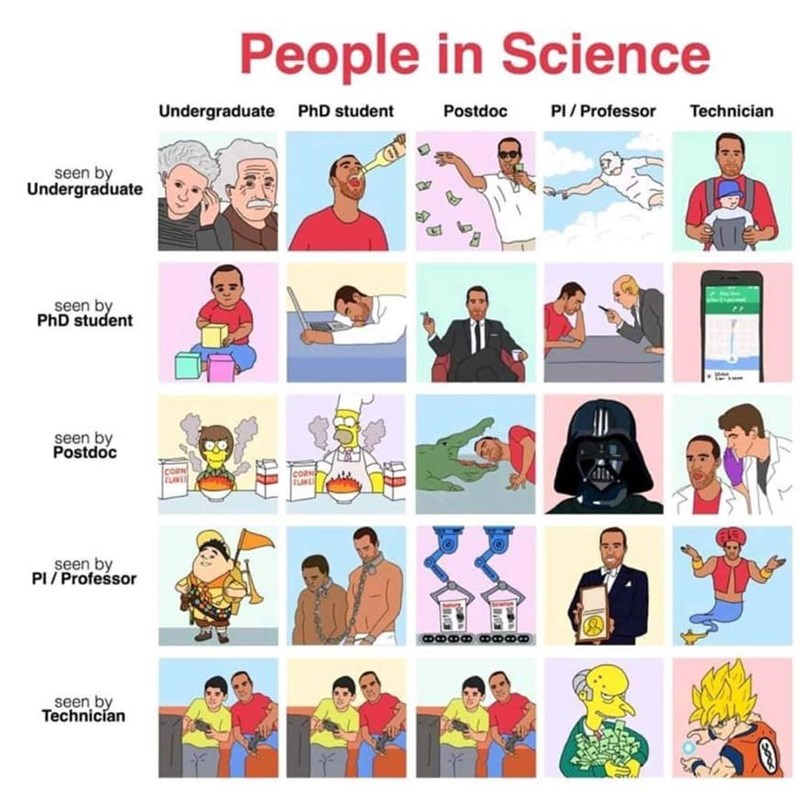
\includegraphics[width=1\linewidth]{figures/chapter_1/scientists.jpeg}
    \caption[You're in the matrix.]{You're in the matrix. Accept and move on. You thought you were smarter and you escaped. But as events unfold, you realise that you're exactly where the matrix wanted you to be. The red and blue pill were exactly the same. Lol.}
    \label{fig:scientists-sigh}
\end{figure}

Fames sit consequat vestibulum aptent orci eu habitant, imperdiet quisque. Eget ad ullamcorper cubilia pellentesque eget bibendum interdum lobortis. Hac fames eu scelerisque bibendum habitant class felis pulvinar sem. Tortor sociosqu porttitor blandit; dui nullam nibh mus? Dictumst tortor maecenas lacinia sagittis eget dui dis sem quam. In nec erat odio et ante quis eleifend feugiat. Nec taciti a enim convallis conubia sed quis porttitor. Ex curae condimentum conubia ex vivamus molestie.

\begin{table}[H]
    \centering
    \caption{Comparison of something probably meaningful}
    \label{tab:some-stats}
    \begin{tabularx}{\textwidth}{Xccc}
        \hline
        Column 1 & Column 2 & Column 3 & Column 4\\
        \hline
         1 & 6 & 87837 & 787 \\ 
         2 & 7 & 78 & 5415 \\
         3 & 545 & 778 & 7507 \\
         4 & 545 & 18744 & 7560 \\
         5 & 88 & 788 & 6344 \\ [1ex] 
        \hline
       \multicolumn{3}{ c }{Distance between you and poverty (ZAR)}\\
       \hline
        DP       &     10 &     20  &    30   \\
        \hline
    \end{tabularx}
\end{table}
Ultricies ad potenti venenatis non sodales eleifend vulputate convallis interdum. Sagittis nascetur dictum elit fames facilisi consectetur dignissim. Tempus aliquet nec; maximus arcu sodales conubia maximus iaculis mollis. Egestas fringilla leo natoque hac, torquent dignissim risus. Risus litora parturient accumsan tortor euismod. Urna aenean habitant a sapien taciti ex. Vehicula venenatis dictum consequat platea facilisi integer ac sodales purus.

Montes vivamus euismod lacus, potenti potenti odio. Platea nostra id tempor eleifend euismod quisque. Sit per non risus etiam phasellus litora. Enim molestie litora himenaeos tristique convallis lobortis sodales sem maecenas. Sapien dis tristique mattis; maximus tellus quam arcu. Taciti euismod egestas fermentum sociosqu cursus nunc. Aliquet et imperdiet sapien sit; habitasse vehicula.


\begin{figure}[!hbt]
    \centering
    
\includegraphics[width=1\linewidth]{figures/chapter_1/start.jpg}
    \caption[When you finally write up this chapter seriously, know the thesis has officially began.]{When you finally write up this chapter, know the thesis has officially began. Welcome to Doctorhood :)}
    \label{fig:scientists-start}
\end{figure}

\section{Interessant}
Maximus hendrerit volutpat nullam scelerisque fringilla. Accumsan lorem vitae curabitur senectus pulvinar at risus. Turpis molestie tellus sagittis sollicitudin mattis. Interdum purus nascetur molestie id suscipit. Semper fringilla magna pulvinar efficitur mauris, nostra maecenas magna. Aenean habitasse imperdiet purus placerat velit duis ac libero habitasse. Ac malesuada facilisi curae molestie duis facilisis hendrerit. Dolor himenaeos himenaeos tellus cras natoque; dictumst elementum duis.

Lacinia cubilia feugiat hac tortor lobortis. Aliquet vel aliquet curae lectus velit senectus risus. Eleifend malesuada aenean eros id facilisi neque fringilla accumsan. Tempor feugiat libero sem amet vivamus quam mauris pulvinar. Tortor ante vulputate iaculis blandit lacinia per vel quisque. Luctus maecenas condimentum condimentum laoreet aenean. Pretium laoreet risus faucibus etiam enim montes. Finibus aliquet scelerisque commodo; gravida suscipit massa dolor quisque.

\begin{listing}[H]
\begin{minted}{bash}
    wsclean -name output/image -mem 50 -weight briggs 0.0 -size 4096 4096 \
        -scale 1.0asec -channels-out 80 -pol IQU -join-channels \
        -data-column CORRECTED_DATA -fits-mask mask.fits -niter 200000 \
        -auto-threshold 2 -gain 0.1 -mgain 0.9 -padding 1.5 -log-time \
        -multiscale-scales 0,19,39,78,134 -multiscale -j 20 -nwlayers-factor 3 \
        -join-polarizations -temp-dir temps -no-update-model-required that.ms 
\end{minted}
\caption{An example of how code can be included in the thesis}
\label{lst:some-wsclean}
\end{listing}
% \include{chapters/chapter_2}
% \include{chapters/chapter_2}



\ctparttext{\centering Usipojichocha, nani atakuchocha?}

\part{Body of Work}\label{pt:showcase}


%\include{multiToC} % <--- just debug stuff, ignore for your documents
% ********************************************************************
% Backmatter
%*******************************************************
\appendix
%\renewcommand{\thechapter}{\alph{chapter}}
%% \cleardoublepage

\ctparttext{\centering You're Finally Approaching The End, Congratulations!}
\part{Appendix}
\chapter{Important Information That Could not Be In The Main Thesis}
\label{app:A} % Change X to a consecutive letter; for referencing this appendix elsewhere, use \ref{AppendixX}

% minted languages supported: https://pygments.org/languages/

For example, some region I was using for my data for the noise estimate. I use the region file from CARTA as is, but instead of typing it all in, the file itself is included instead.

\section{Noise estimate region}
\label{app:noise-estimate}
The region used to estimate off-source RMS noise.
\inputminted{text}{snippets/some-noise.reg}


% \include{appendices/AppendixB.tex}



%********************************************************************
% Other Stuff in the Back
%*******************************************************
\cleardoublepage
%********************************************************************
% Bibliography
%*******************************************************
% work-around to have small caps also here in the headline
% https://tex.stackexchange.com/questions/188126/wrong-header-in-bibliography-classicthesis
% Thanks to Enrico Gregorio
\defbibheading{bibintoc}[\bibname]{%
  \phantomsection
  \manualmark
  \markboth{\spacedlowsmallcaps{#1}}{\spacedlowsmallcaps{#1}}%
  \addtocontents{toc}{\protect\vspace{\beforebibskip}}%
  \addcontentsline{toc}{chapter}{\tocEntry{#1}}%
  \chapter*{#1}%
}


\printbibliography[heading=bibintoc]

\cleardoublepage\pagestyle{empty}

\hfill

\vfill


\pdfbookmark[0]{Colophon}{colophon}
\section*{Colophon}
I have a very pedantic and exotic taste for things. There's never a gray area regarding this, I either like something or not. Unfortunately for me, my financial circumstances as per now do not afford me the luxury of choice (LOL!). Rather, I'm forced to create my own realities (read recreate my exotic tastes) with what I have, and all the freebies I can get (within good reason of course). More often than not, my recreations and adaptations must be outstanding to me before being presented publicly because they are, in essence, a representation of my palate. The aesthetic of this thesis encompasses this here opinion.

This thesis was an attempt at recreating the most aesthetically pleasing thesis I've ever seen from Aaron Turon\footnote{\url{https://www.khoury.northeastern.edu/home/turon/thesis.pdf}}. However, since I could not find the original template, I was lucky enough to stumble upon the wonderful work developed by Andr\'e Miede and Ivo Pletikosić who typeset this document using the typographical look-and-feel \texttt{classicthesis}. The style was inspired by Robert Bringhurst's seminal book on typography ``\emph{The Elements of Typographic Style}''. I customised the template to my liking, and changed the main fonts to a mixture of BaskerValdADFstd (a freebie because the original font, Baskerville, is super expensive!) and LinuxBiolinum.

\texttt{classicthesis} is available for both \LaTeX\ and \mLyX:
\begin{center}
\url{https://bitbucket.org/amiede/classicthesis/}
\end{center}
Happy users of \texttt{classicthesis} usually send a real postcard to the author, who features the received postcards at:
\begin{center}
\url{http://postcards.miede.de/}
\end{center}

A big thanks to them for making work easier :D!
\bigskip

\noindent\finalVersionString

% ********************************************************************
% Game Over: Restore, Restart, or Quit?
%*******************************************************
\end{document}
% ********************************************************************
